% ====================================================================
% JMP_seminar_deck_r11.tex -- V11 outcomes-versus-prospects update.
%
% AUTHORITY
%   docs/normative/JMP_W1_fork_ruling_v1.md, Appendix A (Deputy R1-R7)
%   docs/normative/JMP_W1_BASELINE_F1_authorization_and_Cobs_ruling_v1.md, s5
%
% Certified ex-ante results are reported beside the attained-bundle results.
% Neither welfare perspective is designated primary.
%
% Every numeral comes from \input{deck_numbers_r11}, generated by
% make_deck_numbers_r11.py from three authorized sources only.  No numeral is
% typed on a slide.
% ====================================================================
\documentclass[10pt,aspectratio=169]{beamer}
% ====================================================================
% jmp_beamer_preamble.tex --- shared preamble for the JMP seminar deck.
%
% REUSED VERBATIM from the companion theory talk
%   beamer/reference/Theory_talk/slides/Presentation.tex
%     "Jobs and Well-Being Measurement" (Haydar and Maniquet)
% so that the two decks read as one visual family.  The elements carried
% over unchanged are marked [THEORY-TALK] below; everything else is an
% addition this deck needs and the theory talk does not.
%
% Consistency is the point: same class options, same theme, same accent
% colour, same frame numbering, same appendix handling, same visible-link
% convention, same note-page template, same two-agent sketch palette.
% ====================================================================

% ---- [THEORY-TALK] class, theme and the deep-red accent -------------
\usetheme{metropolis}
\definecolor{deepred}{RGB}{150,25,35}
\setbeamercolor{frametitle}{bg=deepred}
\setbeamertemplate{navigation symbols}{}
% metropolis-defined accents (safe: these beamercolors exist in metropolis)
\setbeamercolor{progress bar}{fg=deepred}
\setbeamercolor{title separator}{fg=deepred}
% frame number as current/total, in deep red
\metroset{numbering=fraction}
\setbeamercolor{footline}{fg=deepred}
% backup appendix: keep the main frame total at the running-order count
\usepackage{appendixnumberbeamer}
% VISIBLE link colours for rehearsal (internal hyperlinks in deep red)
\hypersetup{colorlinks=true,linkcolor=deepred,citecolor=deepred,urlcolor=deepred}

% ---- [THEORY-TALK] encoding, language, maths, tables, tikz ----------
\usepackage[utf8]{inputenc}
\usepackage[english]{babel}
\usepackage{amsmath}
\usepackage{amssymb}
\usepackage{amsfonts}
\usepackage{booktabs}
\usepackage[official]{eurosym}   % \euro --- this deck quotes euro magnitudes
\usepackage{tikz}
\usetikzlibrary{decorations.pathreplacing,arrows.meta,positioning,fit,backgrounds}

% ---- [THEORY-TALK] the two-agent sketch palette --------------------
% red = agent i / household A ; blue = agent h / household B
\definecolor{agenti}{RGB}{200,30,40}
\definecolor{agenth}{RGB}{20,80,200}

% ---- [THEORY-TALK] notes on a second screen (rehearsal view) -------
% The rehearsal build turns this on; the projection build leaves it off.
\usepackage{pgfpages}
% Long notes overflow the note column by default; render them smaller,
% ragged-right, with tight paragraph spacing so the full text stays
% legible and inside the frame on the second screen.
%
% This deck's notes are longer than the theory talk's -- several run past
% one note page at \scriptsize and produced overfull \vbox warnings.  The
% template below keeps the theory talk's look and adds two things it
% needs: \tiny with a tighter baseline, and an \allowbreak-friendly
% vertical box so a long note breaks across note pages instead of
% overflowing.  Hyphenation is relaxed so no line runs into the margin.
\setbeamertemplate{note page}{%
  \vspace{0.3em}\par
  {\tiny\setlength{\parskip}{0.45em}\setlength{\parindent}{0pt}%
   \setlength{\emergencystretch}{3em}%
   \linespread{1.05}\selectfont
   \raggedright\insertnote\par}%
}
% Notes are prose, not code: let TeX hyphenate freely rather than push a
% long word past the measure.
\hyphenpenalty=50
\tolerance=2000

\DeclareMathOperator*{\argmax}{arg\,max}

% ====================================================================
% ADDITIONS for this deck (not in the theory talk)
% ====================================================================

% ---- channel colours ------------------------------------------------
% One colour per decomposition channel, used consistently on every slide
% that names a channel.  Preferences take the theory talk's agent-red so
% the two decks agree on which side of the argument is which.
\definecolor{chpref}{RGB}{200,30,40}     % preferences   (= agenti)
\definecolor{chacc}{RGB}{20,80,200}      % job access    (= agenth)
\definecolor{chearn}{RGB}{200,120,20}    % earning opportunities
\definecolor{chneeds}{RGB}{40,120,70}    % endowments and needs
\definecolor{chenv}{RGB}{60,60,70}       % the whole environment

% ---- the paper's notation ------------------------------------------
% Audience-facing channel names are WORDS on the slides; these commands
% exist so the words are spelled the same way every time they appear.
\newcommand{\pref}{\textcolor{chpref}{preferences}}
\newcommand{\Pref}{\textcolor{chpref}{Preferences}}
\newcommand{\acc}{\textcolor{chacc}{job access}}
\newcommand{\Acc}{\textcolor{chacc}{Job access}}
\newcommand{\earn}{\textcolor{chearn}{earning opportunities}}
\newcommand{\Earn}{\textcolor{chearn}{Earning opportunities}}
\newcommand{\needs}{\textcolor{chneeds}{household endowments and needs}}
\newcommand{\Needs}{\textcolor{chneeds}{Household endowments and needs}}
\newcommand{\env}{\textcolor{chenv}{the environment}}
\newcommand{\Env}{\textcolor{chenv}{The environment}}

% Symbols.  The theory-paper symbols W, z, R, A, y appear ONLY where the
% companion paper is cited; the estimation notation is separate.
\newcommand{\Wmeasure}{W}                      % theory-paper measure
\newcommand{\Jset}{\mathcal{J}}                % theory-paper job space
\newcommand{\Wone}{W^{1}}                      % theory-paper W^1
\newcommand{\yref}{\mathbf{y}^{w}}             % theory-paper reference pay
\newcommand{\gopp}{g}                          % estimated offer density
\newcommand{\uutil}{u}                         % preference index
\newcommand{\Wmm}{\mathrm{W}}                  % money-metric welfare level

% ---- headline / caveat call-outs -----------------------------------
\newcommand{\headline}[1]{{\large\textcolor{deepred}{#1}}}
\newcommand{\caveat}[1]{{\footnotesize\textcolor{deepred}{#1}}}
% a number with its numerical-integration band
\newcommand{\wband}[2]{#1\,\ensuremath{\pm}\,#2}

% ---- the 25-minute variant ------------------------------------------
% Every frame carries \shortdeck (in the 25-minute running order) or
% \longdeck (45-minute only).  \DeckShort, set by the driver file, drops
% the \longdeck frames; the default keeps everything.
%
% The frozen plan's 25-minute running order is 16 slides, reached from the
% 23 by FIVE cuts and TWO merges:
%   CUT   -> backup : 9, 12, 17, 18, 22          (\longdeck)
%   MERGE           : 6+7 -> one slide, 10+11 -> one slide
% So three tags, not two.  A merged pair is written as two full frames for
% the 45-minute deck; in the short deck the SECOND of the pair drops and
% the first shows its merged content.  23 - 5 - 2 = 16.
%
% Usage:  \shortdeck{\begin{frame}...\end{frame}}     kept in both
%         \longdeck{\begin{frame}...\end{frame}}      45-minute only (cut)
%         \mergedaway{\begin{frame}...\end{frame}}    45-minute only (merged)
%         \ifDeckShort ... \else ... \fi              inline merged content
\newif\ifDeckShort\DeckShortfalse
\newcommand{\shortdeck}[1]{#1}                       % always kept
\newcommand{\longdeck}[1]{\ifDeckShort\else#1\fi}    % cut to backup at 25 min
\newcommand{\mergedaway}[1]{\ifDeckShort\else#1\fi}  % folded into the previous
% content shown only in the merged (25-minute) form of a slide
\newcommand{\mergedonly}[1]{\ifDeckShort#1\fi}

% ---- figure helper ---------------------------------------------------
% Every figure is a PDF from the frozen sprint set, included by name from
% beamer/figures/.  \deckfig{name}{width fraction} keeps the call sites
% uniform and makes a missing file fail loudly at compile time.
\graphicspath{{figures/}}
% Heights leave room for the frametitle, the one caption line every figure
% slide carries, and the metropolis footline -- a taller box overflows the
% frame and shows up as an overfull \vbox.
\newcommand{\deckfig}[2]{%
  \begin{center}\includegraphics[width=#2\textwidth,height=0.70\textheight,%
    keepaspectratio]{#1}\end{center}}
\newcommand{\deckfigtwo}[4]{%
  \begin{columns}[c,onlytextwidth]
  \column{0.49\textwidth}\includegraphics[width=\textwidth,height=0.60\textheight,%
    keepaspectratio]{#1}\\{\centering\scriptsize #2\par}
  \column{0.49\textwidth}\includegraphics[width=\textwidth,height=0.60\textheight,%
    keepaspectratio]{#3}\\{\centering\scriptsize #4\par}
  \end{columns}}

% ---- tables ---------------------------------------------------------
% Several slides carry a comparison table that is naturally wider than the
% text block.  \decktable shrinks one to the measure rather than letting it
% run into the margin (an overfull \hbox), and never enlarges a narrow one.
\newcommand{\decktable}[1]{%
  \begin{center}\resizebox{\textwidth}{!}{#1}\end{center}}

\endinput

\input{deck_numbers_r11}
\graphicspath{{figures/}{figures/slides/}{figures/r7/}{figures/r11/}}
\ifdefined\RehearsalDeck
  \setbeameroption{show notes on second screen=right}
\fi
\newcommand{\presenternotesize}{\small}
\setbeamertemplate{note page}{%
  \vspace{0.3em}\par
  {\presenternotesize\setlength{\parskip}{0.45em}\setlength{\parindent}{0pt}%
   \setlength{\emergencystretch}{3em}\linespread{1.05}\selectfont
   \raggedright\insertnote\par}}
\setbeamerfont{frametitle}{size=\normalsize,series=\bfseries}
\setbeamertemplate{frametitle}{%
  \nointerlineskip
  \begin{beamercolorbox}[wd=\paperwidth,sep=0pt]{frametitle}%
    \vskip0.65em
    \hspace*{1.2em}\begin{minipage}{0.91\paperwidth}%
      \raggedright\hyphenpenalty=10000\exhyphenpenalty=10000
      \insertframetitle\par
    \end{minipage}\par
    \vskip0.65em
  \end{beamercolorbox}}
\renewcommand{\caveat}[1]{{\fontsize{8.2}{10}\selectfont\raggedright\color{deepred}#1\par}}
\newcommand{\wfunits}{\caveat{Units: household EUR/month, unequivalised;
  survey weight \texttt{dwt}. Descriptive baseline; no counterfactual,
  no decomposition, no causal reading.}}
\newcommand{\wfunitseq}{\caveat{Units: EUR/month, household-equivalised
  (modified-OECD scale); survey weight \texttt{dwt}. A descriptive dispersion
  comparison, not a welfare-loss index. The modified-OECD scale is used
  throughout the equivalised results.
  Singles and couples equivalised levels are never compared.}}

\title{Unequal Job Opportunities and Well-Being Inequality: A Latent-Jobs Structural Decomposition}
\author{Hisham Haydar}
\date{}

\begin{document}

% ---------------------------------------------------------------- title
\begin{frame}[plain]
\vfill
{\LARGE\bfseries\inserttitle\par}
\vspace{1.3em}
{\color{deepred}\rule{0.80\textwidth}{1pt}}\par
\vspace{1.3em}
{\large Hisham Haydar\par}
LISER and University of Luxembourg\par
\vspace{1.3em}
{\small France, EU-SILC priced through EUROMOD.\par}
\vspace{0.6em}
{\footnotesize Seminar of 17 September. Well-being is measured from two perspectives:
the attained bundle (ATT) and the ex-ante opportunity prospect (EA).\par}
\vfill
\note{Thank you. The question is how much of the inequality in money-metric
well-being is attributable to unequal job opportunities rather than to
differences in taste, and what happens to that attribution when a model
leaves opportunities out. I will show the model, the estimates, the fit, the
welfare definition and a descriptive welfare baseline. The computed preliminary restricted-operator decomposition is in the backup appendix. The certified ex-ante calculation is now reported as a separate perspective beside the attained-bundle measure. The two measures disagree about the dominant channel for single-adult households: earnings dominate the realised job, while access is about three times earnings for the whole prospect. Neither perspective is designated primary.}
\end{frame}

% ================================================================ 1 QUESTION
\section{Question and contribution}

\begin{frame}
\headlineframe{Two people with the same tastes and the same wage need not
face the same set of jobs.}
\vfill
\begin{itemize}\itemsep0.7em
  \item How much of measured welfare inequality is attributable to unequal
        \acc{} and \earn{}, rather than to \pref{}?
  \item What does a model that assumes a common choice set do to that
        attribution?
\end{itemize}
\vfill
\caveat{Both questions are about a \emph{measure}, not about a policy
counterfactual.}
\note{The two questions are the same two questions as in every version of
this paper; nothing in the recent rulings touched them. The first is an
attribution question about a money-metric inequality index. The second is a
methodological question: a discrete-choice labour supply model that gives
every household the same alternatives has to explain non-employment with a
taste parameter, and I want to know whether that relabelling survives into
the welfare accounting.}
\end{frame}

\begin{frame}
\headlineframe{The contribution is a structural opportunity set plus a
welfare measure defined on it.}
\vfill
\begin{itemize}\itemsep0.6em
  \item A random-utility, random-opportunity (RURO) model in which
        \emph{which jobs a household can reach} is estimated, not assumed.
  \item Two money-metric welfare perspectives: the bundle a household
        attains (ATT) and the opportunity prospect it faces (EA).
  \item An exact Shapley decomposition over preferences, geographic/temporal
        access and earning opportunities, holding household resources, needs
        and composition fixed.
\end{itemize}
\vfill
\caveat{The current decomposition equalises preferences, geographic/temporal job access and systematic earning opportunities while holding household resources, needs and composition fixed.}
\note{The contribution has three parts. Preferences and opportunity
components are jointly estimated, with their separation relying on maintained
functional-form and exclusion restrictions. The welfare side asks two questions: how well off a household is in the
bundle it attains, and how valuable the job prospect it faces is. The certified ex-ante calculation is now reported as a separate perspective beside the attained-bundle measure. The two measures disagree about the dominant channel for single-adult households: earnings dominate the realised job, while access is about three times earnings for the whole prospect. Neither perspective is designated primary.}
\end{frame}

% ================================================================ 2 DATA/MODEL
\section{Data and the structural RURO model}

\begin{frame}
\headlineframe{France, EU-SILC priced through EUROMOD: \FrameSingles{}
single-adult and \FrameCouples{} couple households.}
\vfill
\begin{itemize}\itemsep0.6em
  \item Estimation frames: final samples and the current estimated specification.
  \item Estimation frame: each household's observed job plus \FrameDraws{}
        drawn alternatives, every one priced through the tax--benefit system.
  \item Fit diagnostics use a separate, larger panel: \FitNodes{} common
        quadrature nodes per household.
  \item Weights are the survey weights \texttt{dwt} throughout.
\end{itemize}
\vfill
\caveat{Results use a single specification throughout. Estimates from earlier,
non-comparable sample frames are not shown.}
\note{Two estimation samples, singles and couples, on the corrected
criterion-A frames. Everything on the slides after this point is S11. I am
deliberately not showing the older S8 or R240 numbers alongside, because the
frames differ and a side-by-side would invite a comparison the samples do not
support. Each household contributes its observed job and a hundred drawn
alternatives, each of which is run through EUROMOD so the consumption
argument is a real disposable income, not an approximation. The second
number on the slide is a different object: the positive-fit diagnostics
(POSFIT v3b) integrate over a common panel of two thousand and forty-eight
priced quadrature nodes per household, not over the estimation draws.}
\end{frame}

\begin{frame}
\headlineframe{A job is a package; a household draws from its own
distribution over packages.}
\vfill
\begin{center}
\resizebox{\textwidth}{!}{%
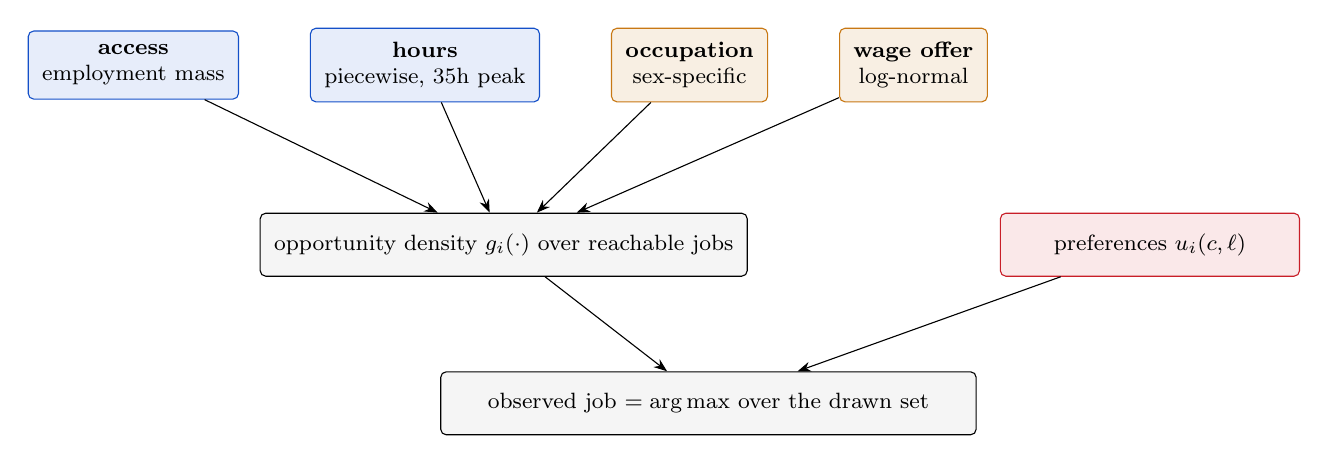
\begin{tikzpicture}[>=Stealth,node distance=9mm,
  box/.style={draw,rounded corners=2pt,align=center,inner sep=5pt,
              font=\footnotesize,minimum height=8mm}]
  \node[box,fill=chacc!10,draw=chacc] (acc) {\textbf{access}\\ employment mass};
  \node[box,fill=chacc!10,draw=chacc,right=of acc] (hrs) {\textbf{hours}\\ piecewise, 35h peak};
  \node[box,fill=chearn!12,draw=chearn,right=of hrs] (occ) {\textbf{occupation}\\ sex-specific};
  \node[box,fill=chearn!12,draw=chearn,right=of occ] (wag) {\textbf{wage offer}\\ log-normal};
  \node[box,fill=black!4,below=14mm of hrs,xshift=10mm,minimum width=52mm] (g)
       {opportunity density $\gopp_i(\cdot)$ over reachable jobs};
  \node[box,fill=chpref!10,draw=chpref,right=32mm of g,minimum width=38mm] (u)
       {preferences $\uutil_i(c,\ell)$};
  \node[box,fill=black!4,below=12mm of g,xshift=26mm,minimum width=68mm] (ch)
       {observed job $=\argmax$ over the drawn set};
  \draw[->] (acc) -- (g); \draw[->] (hrs) -- (g);
  \draw[->] (occ) -- (g); \draw[->] (wag) -- (g);
  \draw[->] (g) -- (ch); \draw[->] (u) -- (ch);
\end{tikzpicture}}
\end{center}
\vfill
\caveat{Access and capability are not separately identified; the access
factor is their product.}
\note{This is the architecture. A job is not an hours cell: it is hours,
occupation and a wage, and whether the household can reach it at all. The
opportunity density factorises into an access margin, a piecewise-constant
hours factor with a peak at the statutory thirty-five hour week, sex-specific
occupation availability, and an occupation-conditioned log-normal wage offer.
Preferences enter separately. The observed job is the argmax over what was
drawn. The identification caveat is on the slide and I keep it there all
talk: the access factor mixes personal capability and market availability and
the cross-section does not separate them.}
\end{frame}

\begin{frame}
\headlineframe{Preferences and the opportunity density are estimated in one
likelihood.}
\slideeq{$\displaystyle
  \Pr(j_i \mid x_i) \;\propto\;
  \exp\!\big\{\, \uutil_i(c_{ij},\ell_{ij}) \;+\; \log \gopp_i(j)
                 \;-\; \log q_i(j) \,\big\}$}
\glossrow{$\uutil$ preferences \quad $\gopp$ estimated opportunity density
\quad $q$ numerical proposal density, divided out}
\vfill
\caveat{The proposal correction is what makes the drawn alternatives a
simulator for the estimated set rather than the choice set itself.}
\note{One likelihood, two structural objects. The proposal density is a
numerical device: the alternatives are drawn from it and it is divided back
out, so it is not part of the economics. That separation matters later,
because the welfare measure I am going to define must not depend on the
proposal density, and I will show that it does not. Preferences and
opportunity components are jointly estimated, with their separation relying
on maintained functional-form and exclusion restrictions. No causal
interpretation follows from that separation. The baseline deliberately keeps
systematic preference heterogeneity parsimonious: age profiles for all four
adult groups and a child-related shifter for women. The child term is
interpreted as a reduced-form behavioural/time-constraint shifter, not as pure
taste. More explicitly, systematic leisure heterogeneity contains an
intercept, age, age squared and group-specific leisure curvature for all four
groups, plus a child shifter for women; sex and household type are carried by
separate parameter blocks.}
\end{frame}

% ================================================================ 3 FIT
\section{Positive estimates and fit}

\begin{frame}
\headlineframe{Estimated model: \SSingActive{} free parameters for
singles, \SCoupActive{} for couples.}
\vfill
\decktable{\begin{tabular}{lrr}
\toprule
 & singles & couples \\
\midrule
free parameters        & \SSingActive{}  & \SCoupActive{} \\
estimation households  & \FrameSingles{} & \FrameCouples{} \\
objective at $\hat\theta$ & \ObjSingles{} & \ObjCouples{} \\
\bottomrule
\end{tabular}}
\vfill
\caveat{Objectives reproduce exactly under an independent diagnostics
reimplementation.}
\note{The headline fact about the estimates is that they are reproducible:
an evaluator built separately for the diagnostics work recovers both stored
objective values to the last digit shown. That is the precondition for
everything on the next two slides. The parameter counts differ because the
couples specification pins nothing at the bound while the singles
specification pins eleven coefficients by construction.}
\end{frame}

\begin{frame}
\headlineframe{Extensive accuracy is reportable for women in each sample;
both groups of men are withheld.}
\slidefig{fitext_r7}
\caveat{The preregistered weighted numerical-adequacy threshold is unchanged.
Single men and coupled men are quadrature-limited; their extensive accuracy is
not reported.}
\note{POSFIT v3b fully re-evaluates the current estimates after rebuilding the
structural band indicators on the priced nodes. The numerical-adequacy rule is
applied mechanically at the unchanged threshold. Single women and coupled
women clear it. Single men and coupled men are quadrature-limited, so their
extensive accuracy is withheld. On the weighted composite decision rule,
conditioning is mechanical stochastic conditioning in all four groups. The
excess-dispersion adjudication is misspecification evidence for the two couple
groups and inconclusive/quadrature-limited for the two single groups. The
earlier three-group excess-predictability claim is withdrawn.}
\end{frame}

\begin{frame}
\headlineframe{The remaining common hours mismatch is the observed 37-hour
mass point, outside structural FT.}
\slidefig{hours37_r7}
\caveat{Underprediction of the observed 37-hour mass point is
\FitGapThirtySevenMinVSeven--\FitGapThirtySevenMaxVSeven{} percentage points
across groups; this is not a structural full-time-band claim.}
\note{The corrected structural bands use the current model definitions. The
observed 37-hour point is isolated as a separate descriptive residual cell,
outside the structural full-time band. Its observed-minus-predicted gap ranges
from \FitGapThirtySevenMinVSeven{} to \FitGapThirtySevenMaxVSeven{} percentage
points. The population MAE is \FitMAESinglesVSeven{} for singles and
\FitMAECouplesVSeven{} for couples. Singles MAE rises slightly, so the correction
is not described as an across-the-board fit improvement. The benchmark audit
also found a RUM-A input-width defect: its alternative-invariant log-density
shift cancels from the conditional likelihood, and RUM-B does not read those
rows, but absolute RUM-A opportunity-mass metadata remain a disclosed
limitation.}
\end{frame}

% ================================================================ 4 KERNEL
\section{Evidence for heterogeneous opportunities}

\begin{frame}
\headlineframe{The access kernel is estimated, and it varies across
households.}
\slidefig{kernelacc_r7}
\caveat{Single-adult estimates; horizontal bars are 1.96 $\times$ CR1 cluster-robust
standard errors. Structural and model-conditional; not causal.}
\note{This is the access block of the estimated opportunity density. The
point is not any individual coefficient, it is that the block is estimated
rather than imposed and that it moves: households in different regional
access environments, and in different survey strata, face materially
different employment masses at the same preferences and the same wage. This
is the evidence that the opportunity side of the model is doing work. It is
also the evidence the welfare measure later rests on, which is why I show it
before the measure and not after.}
\end{frame}

\begin{frame}
\headlineframe{So is the earning-opportunity kernel: an offer distribution,
not a single wage.}
\slidefig{kernelwage_r7}
\caveat{Single-adult estimates; occupation terms shift the offer location.
Dispersion $\hat\sigma=\SElevenWageSigma{}$ ($z=\SElevenWageSigmaZ{}$).}
\note{The wage side is an offer density with an estimated dispersion, not a
point wage attached to each person. Education and experience shift the
location, occupation shifts it again, and the residual dispersion is
precisely estimated. Two households with identical observed wages can have
different earning opportunities in this model, because what they face is a
distribution. That is the second half of what I mean by unequal job
opportunities, and together with the access block it is what the welfare
measure has to be defined on.}
\end{frame}


\begin{frame}
\headlineframe{Two matched men, almost identical tastes, different opportunity
environments.}
\begin{center}
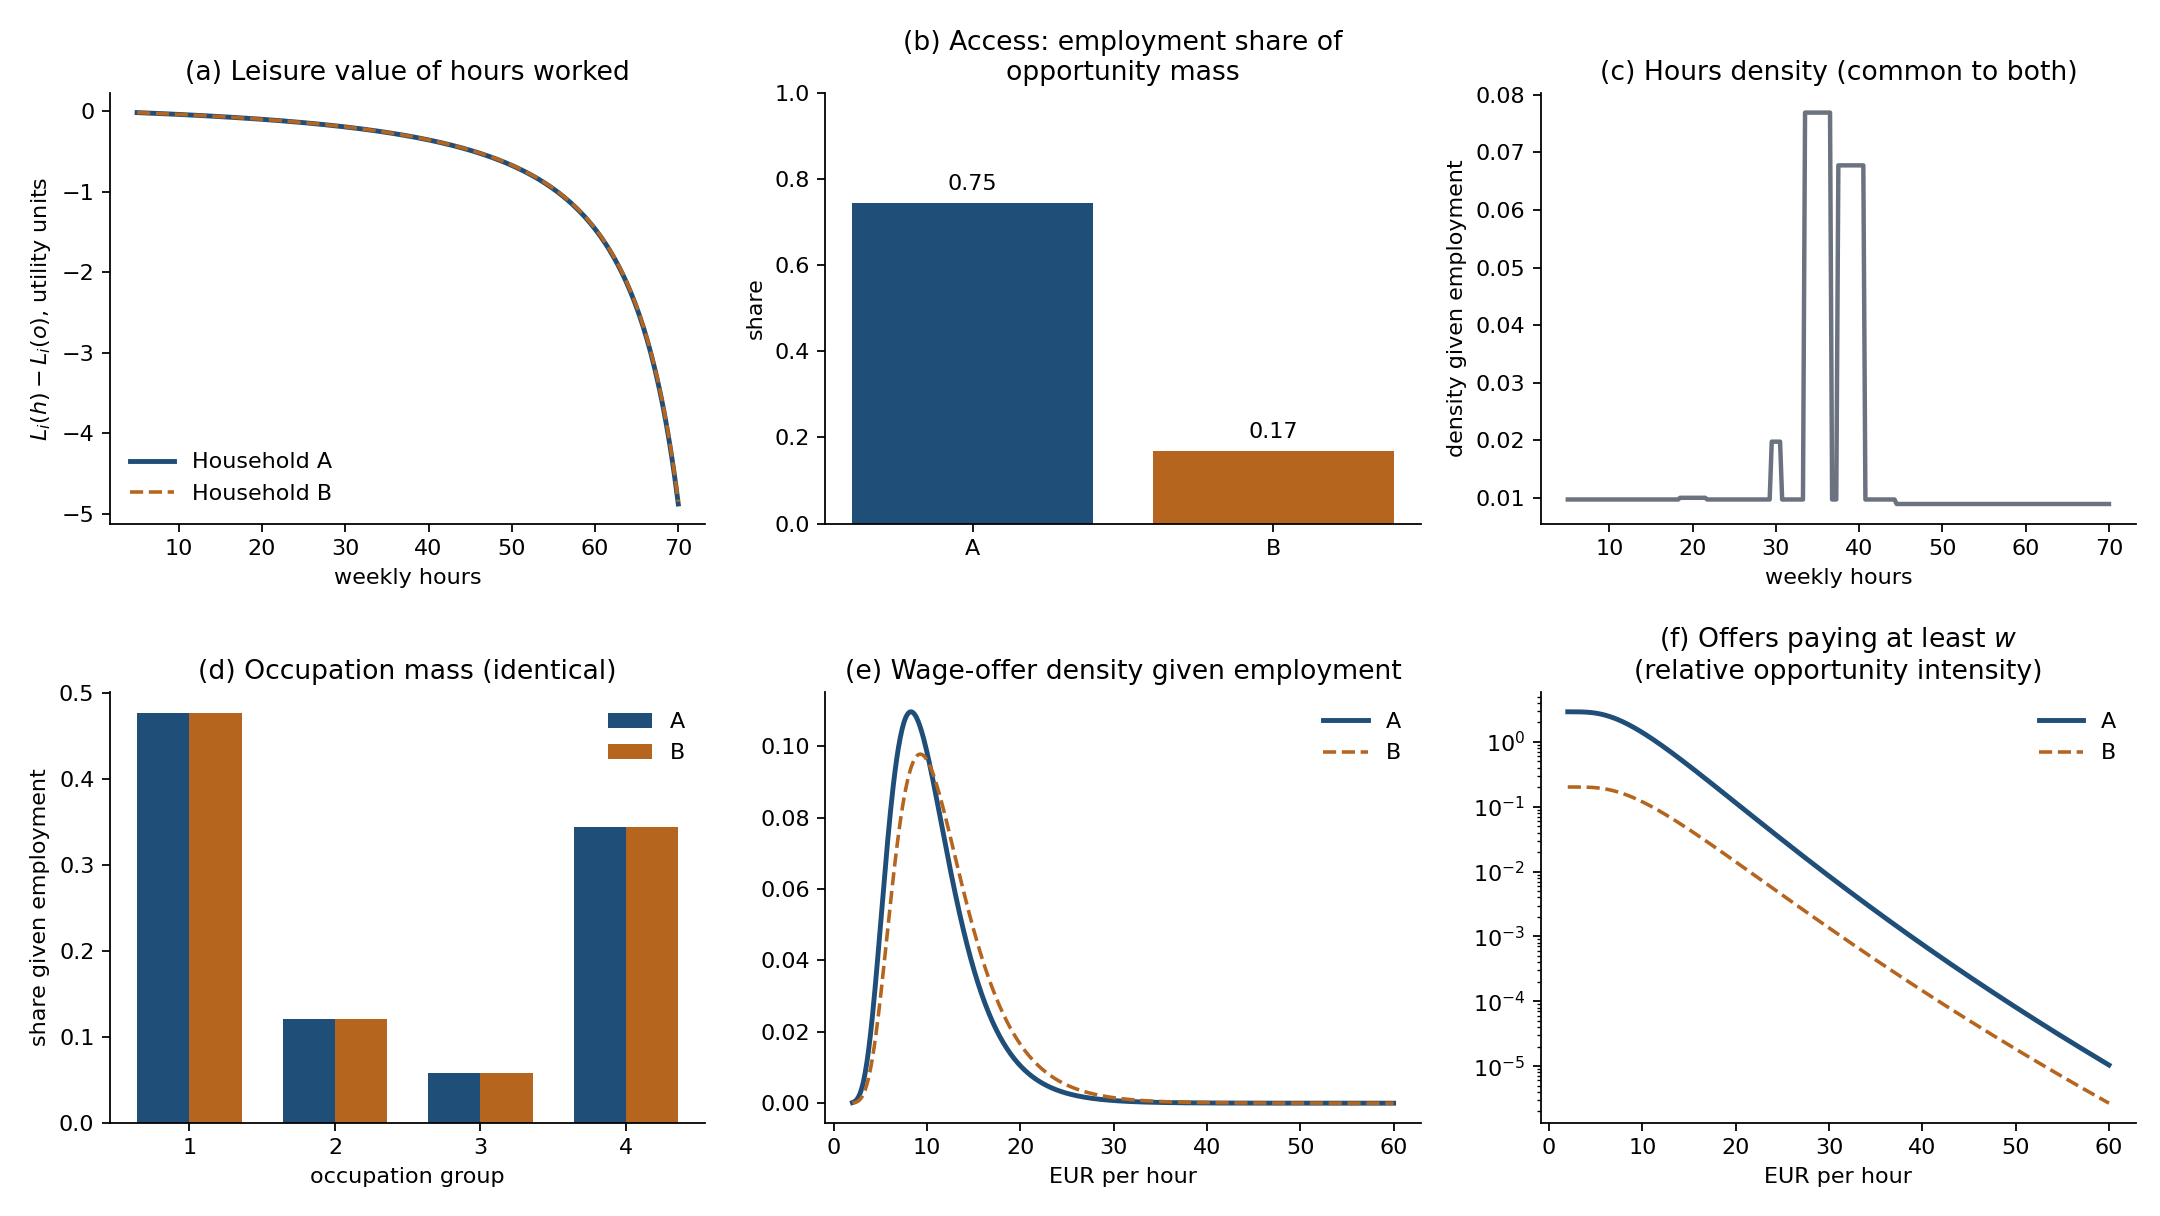
\includegraphics[height=0.64\textheight]{fig_matched_households_v11.png}
\end{center}
\caveat{Same occupation group, hours band and wage quintile. A has
\MatchedAccessRatioREleven{} times B's employment mass; B's wage-offer location
is \MatchedWageGapREleven{} log points higher. A stated-rule teaching example:
not causal, not representative.}
\note{What does unequal opportunity mean in this model? These two single men
look alike in an income table and have nearly identical estimated leisure
profiles. Household A's employment share of opportunity mass is
\MatchedEmpShareAREleven{}, household B's \MatchedEmpShareBREleven{}. B's wage
offers are better: its offer distribution first-order stochastically dominates
A's. But A faces more offers paying at least any given wage over essentially all
offer mass. Hours and occupation opportunities are identical by construction in
this specification. Neither household is better placed on every margin, and
which one is better off depends on the welfare question, which is exactly where
the two perspectives come in.}
\end{frame}

% ================================================================ 5 W1
\section{From choices to well-being: outcomes versus prospects}

\begin{frame}
\headlineframe{ATT: how well off is the household in the bundle it actually
attains?}
\slideeq{$\Wone_i \;=\; m_i(o;z_i)
  \quad\text{where}\quad
  \uutil_i\big(m_i(o),\,o\big) \;=\; \uutil_i(z_i)$}
\glossrow{$z_i$ attained bundle \quad $o$ the non-employment state \quad
$m_i$ the money metric}
\vfill
\caveat{The empirical measure uses the universally available non-employment
state as its reference. A market-job reference is a sensitivity analysis
that requires an unidentified intensity parameter; it is not in the baseline.}
\note{Q\&A note --- ruling R1, JMP\_W1\_fork\_ruling\_v1.md Appendix A.
If asked why this reference and not the market-job reference: the fork
analysis compared Mapping F, the full feasible set including
non-employment, against Mapping M, the market-job universe. R1 rules F
primary for the current paper. M at its dense-law endpoint stops being a
household-specific object and becomes a whole-market reference, and at
finite intensity it needs a set-size parameter the data do not identify.
That is recorded as a limitation and as future work, not as a competing
headline. I am not claiming F is the right reference in the theory; I am
claiming it is the one this empirical specification identifies.}
\end{frame}

\begin{frame}
\headlineframe{Under the current specification $\Wone$ coincides with the
staying-home equivalent --- as a fact about this domain.}
\slideeq{$\Wone_{i,F}
  \;=\; C_i^{\mathrm{obs}}\,
        \exp\!\Big[\tfrac{L_i(j_i^{\mathrm{obs}})-L_i(o)}{\beta_c}\Big]$}
\vfill
\begin{itemize}\itemsep0.4em
  \item Inputs: $C_i^{\mathrm{obs}}$, $L_i(j^{\mathrm{obs}})$, $L_i(o)$,
        $\beta_c$ --- nothing else.
  \item No opportunity density $\gopp$, no proposal $q$, no shock
        $\varepsilon$, no intensity $\kappa$.
  \item Current nonworkers: $W=C$; current workers: $W<C$ under the
        maintained empirical domain.
\end{itemize}
\vfill
\caveat{This is an \textbf{empirical-domain coincidence} under log
consumption and universally available non-employment, not a general
theoretical identity.}
\note{Q\&A note --- ruling R1 and BASELINE-F-1 ruling section 2.
The most likely question here is whether this coincidence is a general
identity. It is not. The coincidence has two ingredients, both specific to what is
estimated: consumption enters utility in logs, and non-employment is
behaviourally available to every household. Change either and the two
measures separate. If asked about the consumption argument: ruling E2
confirms that $C^{\mathrm{obs}}$ must be the exact object entering the
estimated utility at the observed state, not a re-chosen normative income
concept, and the measure-correspondence audit closed that provenance before
the baseline was allowed to run. The empirical Mapping-F implementation evaluates the attained bundle
against the universally available non-employment reference. Under the
current specification, estimated opportunity density therefore affects this
money metric through attained outcomes rather than through a direct
opportunity-prospect term. For a one-nat shortfall,
$L_i(j_i^{\mathrm{obs}})-L_i(o)=-1$, the illustration is
$W=C_i^{\mathrm{obs}}\exp(-1/\beta_c)<C_i^{\mathrm{obs}}$.}
\end{frame}


\begin{frame}
\headlineframe{EA: how valuable is the distribution of job prospects the
household faces?}
\slideeq{$\displaystyle\begin{gathered}
  J_i=\int e^{L_i(j)}\Big(\tfrac{C_i(j)}{\lambda_c}\Big)^{\beta_c}\gopp_i(j)\,d\nu,
  \qquad
  H_i=\int e^{L_i(j)}\gopp_i(j)\,d\nu,
  \\[0.3em]
  W^{EA}_i=\lambda_c\exp\!\Big[\tfrac{\log J_i-\log H_i}{\beta_c}\Big]
  \end{gathered}$}
\vfill
\begin{itemize}\itemsep0.4em
  \item $J_i$: the actual prospect over the whole estimated opportunity environment.
  \item $H_i$: same jobs and availability, equal consumption across jobs.
  \item $W^{EA}_i$: the flat consumption that makes the two prospects equally valuable.
\end{itemize}
\vfill
\caveat{The two measures answer different welfare questions. ATT evaluates the
bundle eventually reached against a common non-employment reference; EA
evaluates the whole distribution of potential job outcomes against a reference
that keeps the opportunity environment and equalises consumption across jobs.}
\note{The second perspective values the prospect itself. Every job enters,
weighted by how available it is and how much the household values it; the
reference keeps exactly those jobs and preferences but pays every job the same.
A common rescaling of the opportunity density cancels, so what matters is how
opportunity weight is spread across jobs. Neither perspective corrects the
other. Under the extreme-value shocks, log J is the expected utility of the best
reachable job up to a constant, so the measure treats taste-shock variety as
welfare-relevant; that is a normative position, and I flag it. The ex-ante
calculation passed all its numerical checks; that certifies the computation,
not causal identification, parameter uncertainty or normative uniqueness.}
\end{frame}

% ================================================================ 6 BASELINE
\section{Attained-bundle distribution, equivalised}

\begin{frame}
\headlineframe{Baseline $\Wone$-F, equivalised, single adults.}
\vfill
\decktable{\begin{tabular}{lrr}
\toprule
 & $C^{\mathrm{eq}}$ & $\Wone_{F}{}^{\mathrm{eq}}$ \\
\midrule
households        & \WFSingN{}         & \WFSingN{} \\
weighted mean      & \WFSingCEqMean{}   & \WFSingWEqMean{} \\
weighted median    & \WFSingCEqMedian{} & \WFSingWEqMedian{} \\
weighted Gini      & \WFSingCEqGini{}   & \WFSingWEqGini{} \\
\bottomrule
\end{tabular}}
\vfill
\wfunitseq
\caveat{The sample aggregates reproduce to machine precision under an
independent reimplementation. This is a descriptive dispersion comparison
($C^{\mathrm{eq}}$ against
$\Wone_F{}^{\mathrm{eq}}$ within the singles sample), not a welfare-loss
index.}
\note{Q\&A note --- BASELINE-F-1 ruling, E3-EQ, and ruling R7.
Equivalised results are primary on this slide: the household-equivalised
Gini of $\Wone_F$ is below the household-equivalised Gini of observed
consumption, for singles. I show that as a descriptive dispersion
comparison only, not as a welfare-loss statement --- the ratio
$\Wone_F/C^{\mathrm{obs}}$ reflects the systematic leisure term at the
observed job relative to home leisure, not a monetary loss, and I am not
constructing a loss index on this slide. The equivalence scale is the
modified-OECD scale, ratified as the primary scale for current JMP
distributional reporting by the Deputy ruling ``SCALE CLOSED; CHILD-SHIFTER
FRAMING'', section 1, on the economics review in
JMP\_SCALE\_REVIEW\_1\_equivalence\_scale\_economics\_v1.md; the scale
question is closed. The unequivalised construction this equivalises is
unchanged and is in the backup appendix.}
\end{frame}

\begin{frame}
\headlineframe{Baseline $\Wone$-F, equivalised, couples.}
\vfill
\decktable{\begin{tabular}{lrr}
\toprule
 & $C^{\mathrm{eq}}$ & $\Wone_{F}{}^{\mathrm{eq}}$ \\
\midrule
households        & \WFCoupN{}         & \WFCoupN{} \\
weighted mean      & \WFCoupCEqMean{}   & \WFCoupWEqMean{} \\
weighted median    & \WFCoupCEqMedian{} & \WFCoupWEqMedian{} \\
weighted Gini      & \WFCoupCEqGini{}   & \WFCoupWEqGini{} \\
\bottomrule
\end{tabular}}
\vfill
\wfunitseq
\caveat{Reported separately from singles: no pooled figure, and no
cross-sample level comparison is drawn on this slide or elsewhere in this
deck. The same independently reimplemented welfare construction and
equivalence scale are used as for single adults.}
\note{Q\&A note --- BASELINE-F-1 ruling, E3-EQ, and ruling R7.
Same descriptive comparison, on the couples sample. I am deliberately not
placing this table next to the singles one: the two are separate estimation
frames, the welfare unit differs, and R7 forbids presenting a singles/couples
equivalised-level comparison as a finding. If asked how the couples numbers
compare to singles, the honest answer is that this deck does not draw that
comparison, and I would want to see it examined outside a seminar slide
before treating it as informative. The scale is the same ratified
modified-OECD scale as on the singles slide (Deputy ruling ``SCALE CLOSED;
CHILD-SHIFTER FRAMING'', section 1); ratifying the scale does not license a
cross-sample level comparison.}
\end{frame}


% ============================================================ V9 COMPARISON
\begin{frame}
\headlineframe{The welfare question changes which labour-market inequality matters.}
\vspace{0.2em}
\begin{columns}[T,onlytextwidth]
\begin{column}{0.485\textwidth}
\begin{beamercolorbox}[rounded=true,sep=0.8em]{block body}
{\bfseries ATT: the attained bundle}\par\smallskip
\decktable{\begin{tabular}{lcc}
\toprule
& raw & equivalised \\
\midrule
single adult & \AttOppSinglesRawRNine\% & \AttOppSinglesEqRNine\% \\
couple       & \AttOppCouplesRawRNine\% & \AttOppCouplesEqRNine\% \\
\bottomrule
\end{tabular}}
\smallskip
{\color{chearn}\bfseries Earning opportunities $>$ access}\\
in both populations and at both scales.
\end{beamercolorbox}
\end{column}
\begin{column}{0.485\textwidth}
\begin{beamercolorbox}[rounded=true,sep=0.8em]{block body}
{\bfseries EA: the whole opportunity prospect}\par\smallskip
\decktable{\begin{tabular}{lcc}
\toprule
& raw & equivalised \\
\midrule
single adult & \EAOppSinglesRawRNine\% & \EAOppSinglesEqRNine\% \\
couple       & \EAOppCouplesRawRNine\% & \EAOppCouplesEqRNine\% \\
\bottomrule
\end{tabular}}
\smallskip
{\color{chacc}\bfseries Singles: access $\simeq 3\times$ earnings;}\\
couples: no reversal, earnings $>$ access.
\end{beamercolorbox}
\end{column}
\end{columns}
\vfill
\caveat{The importance assigned to different labour-market inequalities
depends on whether welfare evaluates the realised outcome or the opportunity
prospect itself. Cells: access plus earning opportunities as a share of each
perspective's own baseline Gini, holding resources, needs and composition fixed.
Neither perspective is designated primary.}
\note{This is the comparison to remember. The attained-bundle measure asks what
the realised job is worth; earning opportunities dominate because wages drive
disposable consumption at that job. The ex-ante measure asks what the whole job
prospect is worth; reachability therefore enters directly, and for single-adult
households access is \EAAccessRatioSinglesRawRNine{} times earnings before
equivalisation and \EAAccessRatioSinglesEqRNine{} times after it. For couples,
equivalisation is materially consequential: the ex-ante access-plus-earnings
share moves from \EAOppCouplesRawRNine{} to \EAOppCouplesEqRNine{} per cent and
the preference contribution turns negative. I make no directional preference
claim and do not designate either welfare perspective as primary. All cells
come from a restricted accounting that holds resources, needs and composition
fixed; they are not causal or total opportunity shares.}
\end{frame}

% ================================================================ 7 ARCHITECTURE
\begin{frame}
\headlineframe{What I would like from you today.}
\vfill
\begin{itemize}\itemsep0.7em
  \item Is universally available non-employment the reference you would want
        for this question?
  \item Which counterfactual attainment estimand would you defend?
  \item What would convince you the access kernel is identified, given that
        access and capability are not separated?
\end{itemize}
\vfill
\caveat{Thank you.}
\note{Q\&A note --- rulings R1, R5, and the identification caveat carried
from the model slide. Three questions, in the order I most need answers. The
reference domain choice is normative and I would like it challenged. The
attainment estimand is the blocking design decision. And the access
identification caveat is the one every discussant raises; I would rather hear
what evidence would settle it than defend the current position.}
\end{frame}

% ================================================================ BACKUP
\appendix

\begin{frame}
\headlineframe{Preliminary restricted-operator decomposition}
\vfill
{\small The attained-bundle and ex-ante decompositions apply the same restricted three-pathway game while holding resources, needs and composition fixed. The ex-ante calculation is numerically certified; the attained-bundle counterfactual remains preliminary. Neither is a comprehensive or causal share of inequality due to all opportunities.\par}
\vfill
\note{The attained-bundle and ex-ante decompositions apply the same restricted three-pathway game while holding resources, needs and composition fixed. The ex-ante calculation is numerically certified; the attained-bundle counterfactual remains preliminary. Neither is a comprehensive or causal share of inequality due to all opportunities.}
\end{frame}



\begin{frame}
\headlineframe{This bounded decomposition equalises three channels, not whole job access.}
\vfill
\begin{itemize}\itemsep0.6em
  \item[$P$] systematic utility heterogeneity (tastes + reduced-form time
        constraints) $\rightarrow$ common reference
  \item[$A$] local geographic/temporal access shifters
        (region, urban/rural, year) $\rightarrow$ common reference
  \item[$B$] wage-offer location $\rightarrow$ common reference location
\end{itemize}
\vfill
\caveat{Household resources, needs and composition are held fixed; adding them
as a fourth pathway $D$ is a planned extension, and $A+B+D$ would not be an
opportunity share. Personal occupation access and hours-band access are not
equalised by $A$.}
\note{Q\&A note --- ruling R7 and final economics review M5.
For DECOMP-2, $A$ is local geographic/temporal access shifters (region,
urban/rural, year). It is not personal occupation access, hours-band access
or full job access. Children enter the current structural specification
through a reduced-form female time-constraint shifter. In a unitary
labour-supply model this term may capture both tastes and
childcare/home-production constraints; we therefore do not interpret it as
pure preference heterogeneity. The baseline deliberately keeps systematic
preference heterogeneity parsimonious: age profiles for all four adult groups
and a child-related shifter for women. The child term is interpreted as a
reduced-form behavioural/time-constraint shifter, not as pure taste.}
\end{frame}

\begin{frame}
\headlineframe{The bounded decomposition is executed; the final attainment estimand remains
under design.}
\vfill
\begin{center}
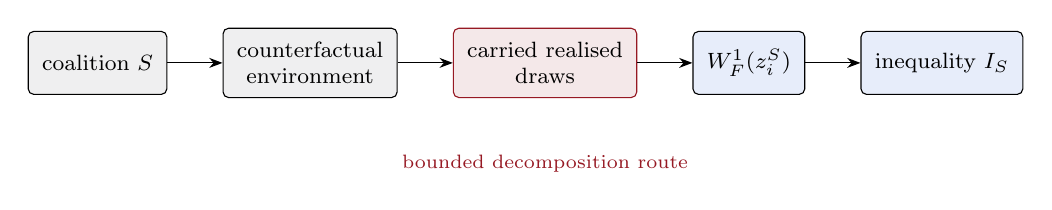
\begin{tikzpicture}[>=Stealth,node distance=7mm,
  b/.style={draw,rounded corners=2pt,align=center,font=\footnotesize,
            inner sep=5pt,minimum height=8mm}]
  \node[b,fill=chenv!8] (s) {coalition $S$};
  \node[b,fill=chenv!8,right=of s] (e) {counterfactual\\environment};
  \node[b,fill=deepred!10,draw=deepred,right=of e] (z) {carried realised\\draws};
  \node[b,fill=chacc!10,right=of z] (w) {$\Wone_F(z_i^{S})$};
  \node[b,fill=chacc!10,right=of w] (i) {inequality $I_S$};
  \draw[->] (s) -- (e); \draw[->] (e) -- (z);
  \draw[->] (z) -- (w); \draw[->] (w) -- (i);
  \node[below=6mm of z,font=\scriptsize,color=deepred,align=center]
       {bounded decomposition route};
\end{tikzpicture}
\end{center}
\vfill
\caveat{This exercise reuses the already-priced estimation panel with no
re-estimation and no new pricing. The final decomposition's
counterfactual-attainment estimand remains under design.}
\note{Q\&A note --- ruling R5 and final economics review M10.
The preliminary exercise carries the household's realised draws through each
counterfactual environment. That is an executed, bounded accounting route,
not the final counterfactual-attainment estimand. The final design still has
to choose between a realised-bundle route with conditioned latent
heterogeneity and an ex-ante $g$-computation route; the inequality of expected
welfare is not the expected inequality of welfare.}
\end{frame}

% ================================================================ 8 WIP


\begin{frame}
\headlineframe{Preliminary restricted-operator decomposition}
\vfill
{\small
In a preliminary three-factor structural exercise that holds household
resources, needs and composition fixed, equalising systematic utility
heterogeneity, coarse geographic/temporal access heterogeneity and earning
opportunities changes money-metric well-being inequality by
\DTwoMinPct--\DTwoMaxPct\% of the baseline Gini, depending on household type
and reporting scale. Within the Shapley allocation of that movable component,
earning-opportunity heterogeneity has a larger contribution than the coarse
geographic/temporal access channel in both samples and both reporting
conventions. The preference contribution is not sign-robust to
equivalisation. This percentage is the change generated by the declared restricted P/A/B game. It is not an estimate of the total fraction of inequality caused by unequal job opportunities.\par}
\vfill
\caveat{These are preliminary model-based accounting results, not causal
estimates and not the final decomposition of total well-being inequality.}
\note{Q\&A note --- ruling R7 and final economics review M3--M11.
The decomposition is bounded by design because household resources, needs
and composition are held fixed. Within that bounded game, equalising P/A/B
changes the Gini by \DTwoMinPct--\DTwoMaxPct\% of its baseline level, depending
on sample and reporting scale. The restriction is by construction; the
realised numerical magnitude is a model result under that restriction.
Dispersion in consumption is quantitatively large relative to dispersion in
log well-being: Var(log C) is roughly
\DTwoVarMinPct--\DTwoVarMaxPct\% of Var(log W), with the excess offset by a
large negative covariance between consumption and the leisure valuation.
DECOMP-2 holds household resources, needs and composition fixed, leaving
important sources of dispersion outside the P/A/B allocation. If asked about
wage elasticities: a valid gross-wage perturbation requires new tax-benefit
repricing over the affected job alternatives, and the current priced support
does not contain that counterfactual. This percentage is the change generated by the declared restricted P/A/B game. It is not an estimate of the total fraction of inequality caused by unequal job opportunities. The preliminary attainment exercise is evaluated on the already-priced estimation panel. That panel sparsely represents the lower part of the structural hours support. A separate integration audit shows substantial structural mass in that region. The direct importance of this limitation for the current attained-bundle decomposition has not been fully quantified, so the result remains explicitly preliminary.}
\end{frame}

\begin{frame}
\headlineframe{The earnings operator equalises wage-offer location only.}
\vfill
{\small The earning-opportunity channel equalises wage-offer location only: the systematic differences associated with education and potential experience, which shift offer locations by at most about \OfferLocationLog{} log points. The common offer spread (about \OfferSpreadLog{} log points), wage-draw luck and selection remain in the residual and are quantitatively larger than the location differences removed by this operator. This is a definitional boundary of the exercise, not a measurement error. Equalising locations can change attained wages; it does not equalise the whole wage distribution. The diagnostic comparison that also compresses the common spread and selection is a bound, not an additional decomposition result. Thin effective support for couples leaves individual wage attainment noisy and remains a numerical limitation.\par}
\vfill
\note{The earning-opportunity channel equalises wage-offer location only: the systematic differences associated with education and potential experience, which shift offer locations by at most about \OfferLocationLog{} log points. The common offer spread (about \OfferSpreadLog{} log points), wage-draw luck and selection remain in the residual and are quantitatively larger than the location differences removed by this operator. This is a definitional boundary of the exercise, not a measurement error. Equalising locations can change attained wages; it does not equalise the whole wage distribution. The diagnostic comparison that also compresses the common spread and selection is a bound, not an additional decomposition result. Thin effective support for couples leaves individual wage attainment noisy and remains a numerical limitation.}
\end{frame}


\begin{frame}
\headlineframe{Baseline $\Wone$-F, unequivalised, single adults
(verification backup).}
\vfill
\decktable{\begin{tabular}{lr}
\toprule
households                    & \WFSingN{} \\
weighted mean                 & \WFSingMean{} \\
weighted median               & \WFSingMedian{} \\
weighted Gini                 & \WFSingGini{} \\
\midrule
observed workers              & \WFSingWorkers{} \\
observed non-workers          & \WFSingNonworkers{} \\
\bottomrule
\end{tabular}}
\vfill
\wfunits
\caveat{Secondary/verification slide: the equivalised singles slide (\S6) is
primary. The sample aggregates reproduce to machine precision under an
independent reimplementation.}
\note{This is the literal observed-bundle Mapping-F distribution before
equivalisation, kept here so any question about the un-scaled level or about
worker/non-worker counts has a one-slide answer. It is not the headline: the
equivalised slide in \S6 is. For non-workers the measure equals observed
consumption exactly by construction; for workers it is strictly below it.}
\end{frame}

\begin{frame}
\headlineframe{Baseline $\Wone$-F, unequivalised, couples
(verification backup).}
\vfill
\decktable{\begin{tabular}{lr}
\toprule
households                    & \WFCoupN{} \\
weighted mean                 & \WFCoupMean{} \\
weighted median               & \WFCoupMedian{} \\
weighted Gini                 & \WFCoupGini{} \\
\midrule
observed workers              & \WFCoupWorkers{} \\
observed non-workers          & \WFCoupNonworkers{} \\
\bottomrule
\end{tabular}}
\vfill
\wfunits
\caveat{Secondary/verification slide: the equivalised couples slide (\S6) is
primary. Reported separately from singles. No pooled figure: the two samples
are separate estimation frames and the welfare unit differs.}
\note{The couples backup is on its own slide and there is no pooled row:
the two samples are separate estimation frames with different welfare
units, and even on the ratified modified-OECD scale this deck never compares
singles and couples levels. These are unequivalised household totals:
couples pool two earnings streams, and the non-employment count is small.
The pricing-floor issue that affects the neither-work bundle for a subset of
couples does not enter here, because this baseline is evaluated at the
observed bundle and never prices the home state.}
\end{frame}

\begin{frame}
\headlineframe{Pre-registered checks for the baseline $\Wone$-F measure}
\vfill
\decktable{\begin{tabular}{lll}
\toprule
check & singles & couples \\
\midrule
non-workers, $\max|\Wone-C^{\mathrm{obs}}|$ & \WFSingCone{} & \WFCoupCone{} \\
workers, ratio outside $(0,1)$              & \WFSingCtwo{} & \WFCoupCtwo{} \\
dependency test ($\gopp,q,\varepsilon,\kappa$) & PASS & PASS \\
worked-household correspondence test            & PASS & PASS \\
indifference identity, $\max|\Delta \uutil|$ & \WFSingCfive{} & \WFCoupCfive{} \\
guards triggered                            & 0 & 0 \\
\bottomrule
\end{tabular}}
\vfill
\caveat{All six checks were pre-registered before execution. Worker-ratio
violations were to be explained, never clipped; none occurred.}
\note{The checks are the reason the baseline is presentable. C1 and C2 are
the model-implied domain conditions. C3 is the dependency test: the baseline
API accepts no opportunity density, no proposal, no shock and no intensity,
and does not read them indirectly. C5 inverts the utility numerically and
confirms the indifference identity to machine precision.}
\end{frame}

\begin{frame}
\headlineframe{Quadrature adequacy for extensive-margin accuracy}
\vfill
\decktable{\begin{tabular}{lrl}
\toprule
group & extensive accuracy & status \\
\midrule
coupled women & \FitExtCF{}\% & reported (ratio \FitExtRatioCF{}) \\
single women  & \FitExtSF{}\% & reported (ratio \FitExtRatioSF{}) \\
coupled men   & ---           & quadrature-limited, withheld \\
single men    & ---           & quadrature-limited, withheld \\
\bottomrule
\end{tabular}}
\vfill
\caveat{Weighted, all households. Ratio is Monte Carlo s.e. over sampling
s.d.; the pre-registered criterion is $\le 0.25$. Node bootstrap over
\FitNodes{} common quadrature nodes per household (diagnostic panel, not the
estimation draws). Simulated bands: \FitSims{} outcome vectors at fixed
$\hat\theta$. Source: individual-level predictive diagnostics.}
\note{The gate was fixed before the statistics were computed. It asks
whether numerical integration error is small enough relative to sampling
variation for the statistic to be a statement about the model rather than
about the quadrature. Withholding rather than downgrading is deliberate:
a quadrature-limited number carries no information about fit.}
\end{frame}

\begin{frame}
\headlineframe{Scope of the welfare evidence shown here}
\vfill
\decktable{\begin{tabular}{ll}
\toprule
question & treatment here \\
\midrule
empirical reference & home is selected on this empirical domain \\
alternative welfare construction & excluded from the baseline \\
measure correspondence & verified for worked households \\
counterfactual attainment & in design, not executed \\
reported scope & descriptive baseline and bounded preliminary decomposition \\
observed consumption & the estimated utility's own argument \\
alternative consumption benchmark & not constructed or reported \\
equivalised reporting & primary (\S6), using the modified-OECD scale \\
\bottomrule
\end{tabular}}
\vfill
\caveat{Supporting technical provenance is retained in the source-only
provenance block.}
\note{This backup slide exists so that any question of the form ``why is
that not here'' has a one-line answer with a document behind it.}
\end{frame}

% BEGIN READER-VOICE PROVENANCE
% Source-only provenance; excluded from rendered reader text.
% Specifications: S11; artifact s11_welfare_specs_of_record_v1.json; SHA-256
% 5FDC88502493CE540B088880EECF049BC268392FF3E8790FFE78A16AA6DDC884.
% Welfare definition: Mapping F; artifact JMP_W1_fork_ruling_v1.md; Deputy
% ruling R1; SHA-256
% 7F5D26857D8A96174A9924848F65A02611944273D7775FDC52DC82364A818C05.
% Welfare authorization: BASELINE-F-1 and E1; artifact
% JMP_W1_BASELINE_F1_authorization_and_Cobs_ruling_v1.md; SHA-256
% 54DFD886E41D0A89C1056CBEA5FA51E0A1294D3CA0813F938802BDC3DBD9EE0E.
% Welfare aggregates: artifact baseline_f1_verification_v1.md; MNL commit
% 6048c9f7; independent verification b5550af5; SHA-256
% DA7BADF639F3D502D47B301558453D76501C9C44033ECE3F17BDE350BFD5E55F.
% Equivalised reporting: E3-EQ; artifact
% JMP_BASELINE_F1_equivalised_reporting_v1.md; commit 4c4e07e; scale ruling
% "SCALE CLOSED; CHILD-SHIFTER FRAMING", s1; artifact
% JMP_SCALE_REVIEW_1_equivalence_scale_economics_v1.md; SHA-256
% 7CACE61E4476148D05C894729F05FF38F79AF803B9E637449EC76F9CB808014E.
% Predictive diagnostics: POSFIT v3b; repository MNL_posfit; branch
% diagnostics/posfit-v3; commit cd7247cf; evaluator commit 55bb0d0; artifact
% run_provenance.json; SHA-256
% 34A4EC87ED1C4218984961BB3493062B4281DB2C42437B47DA01A78973380E58.
% Bounded decomposition: DECOMP-2; repository MNL_decomp; branch
% welfare/preseminar-pab; commit b52761b4; artifact
% preseminar_pab_record_v1.json; SHA-256
% BCBE4B6FC742DAA39535D5C3EB03BDA0641055A9F5E851B4F53F62FA3E612011.
% Diagnostic boundary: DECOMP-DIAG-1; docs/Decomposition_diag_1.txt; SHA-256 EAD1B7C8243FE1498F00DCF287331BEEC94165332AA3BB64041A0F645D339A74; location and common spread in log points.
% Presentation: REPORT-V6; all decomposition frames after appendix.
% END READER-VOICE PROVENANCE

\end{document}
